%%%%%%%%%%%%%%%%%%%%%%%%%%%%%%%%%%%%%%%%%%%%%%%%%%%%%%%%%%%%%%%%%%%%%%
%%                           SECTION III
%%%%%%%%%%%%%%%%%%%%%%%%%%%%%%%%%%%%%%%%%%%%%%%%%%%%%%%%%%%%%%%%%%%%%



\chapter{Results}

%%%%%%%%%%%%%%%%%%%%%%%%%%%%%%%%%%%%%%%%%%%%%%%%%%%%%%%%%%%%%%%%%%%%%%%%%%%%%%%%%%%%%%%%%%%%%%%%%%%%
\section{Preliminary results}
%%%%%%%%%%%%%%%%%%%%%%%%%%%%%%%%%%%%%%%%%%%%%%%%%%%%%%%%%%%%%%%%%%%%%%%%%%%%%%%%%%%%%%%%%%%%%%%%%%%%

At this point, four separate methods for \qoi calculation have been discussed; forward and adjoint inner products for both Sn and VET formulations. When dealing with sensitivity measurements, the forward solutions are expected to give the most exact answer simply because it involves an additional forward solve of the perturbed system for each perturbation case. The adjoint methods for sensitivity are relying on a first-order approximation (we dropped the double $\delta$ terms), however they only require a single forward solve and a single adjoint for use with all perturbation cases. 

The four methods were implemented in a MATLAB finite element method (FEM) solver. One-dimensional test cases were run, varying which parameter experienced perturbation and the magnitude of the perturbation. The results of the four different sensitivity methods were analyzed to identify cases where the efficient VET adjoint showed promise as a time and memory efficient method for computing sensitivity. As a representation of this, the \% \qoi response is plotted against the \% change in a given parameter $p$, which are defined as
\begin{subequations}
\begin{equation}
\text{\% \qoi response}=\frac{\delta \qoi}{\qoi} \,,
\end{equation}
\begin{equation}
\text{$p$ \% change}=\frac{\delta p}{p} \,.
\end{equation}    
\end{subequations}

%%%%%%%----------------------------------------------------------------------------------------------
\subsection{Homogeneous System, Uniform Perturbations}
%%%%%%%----------------------------------------------------------------------------------------------
The first test case consisted of a 1D homogeneous system, with a volumetric source throughout. The width of the system was 10 (arbitrary units). Solutions were obtained using a 200 element mesh. Three systems of varying initial cross sections $\sigt$ and $\sigs$ were tested. Perturbations in $\sigt$, $\sigs$, and $\scalSource$ to the system were made uniformly, resulting in the perturbed system remaining homogeneous. The desired \qoi is the total flux in the middle fifth of the system.
\todo{Add in incident flux perturbations. In the unperturbed state, the incident flux is 0, so we cant use a \% perturbation and will instead have to opt for an absolute perturbation}

\begin{figure}[H]
\label{HomoPertt}
\centering
\begin{subfigure}{.5\textwidth}
  \centering
  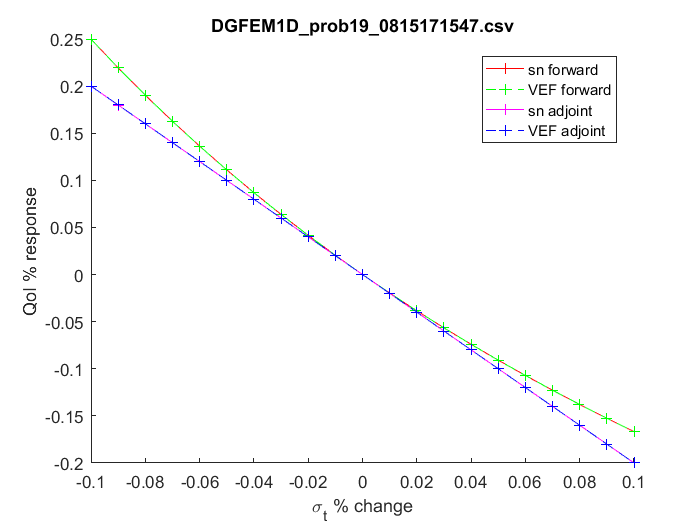
\includegraphics[width=.98\linewidth]{figures/19sigtSens.png}
  \caption{Unperturbed state: $\sigt=2$, $\sigs=1$. }
  \label{fig:sfig1}
\end{subfigure}%
\\
\begin{subfigure}{.5\textwidth}
  \centering
  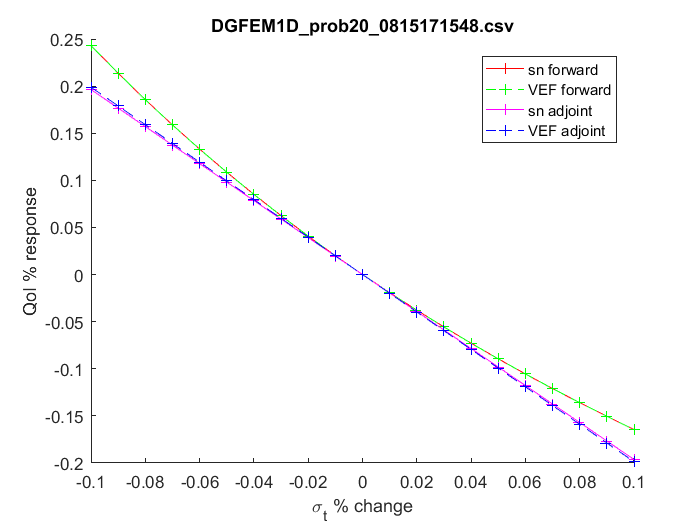
\includegraphics[width=.98\linewidth]{figures/20sigtSens.png}
  \caption{Unperturbed state: $\sigt=1$, $\sigs=0.5$. }
  \label{fig:sfig2}
\end{subfigure}
\\
\begin{subfigure}{.5\textwidth}
  \centering
  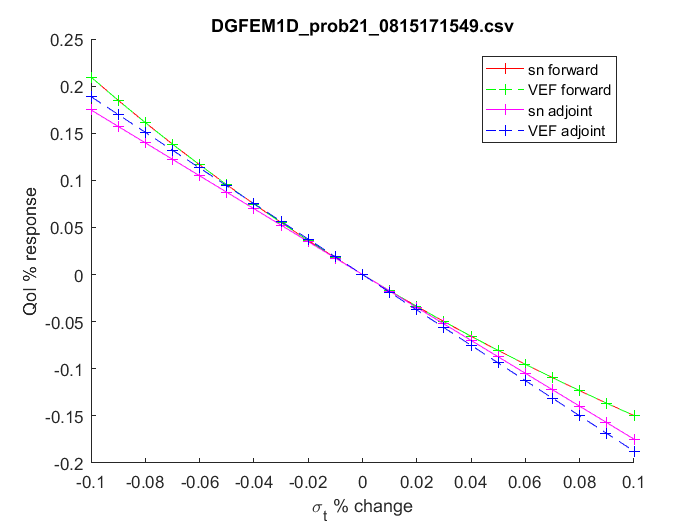
\includegraphics[width=.98\linewidth]{figures/21sigtSens.png}
  \caption{Unperturbed state: $\sigt=0.5$, $\sigs=0.25$.}
  \label{fig:sfig3}
\end{subfigure}
\caption{Plots of $\sigt$ perturbation sensitivity for a uniform perturbation in a homogeneous system.}
\label{fig:fig}
\end{figure}

\jcr{change the other figures/caption in the same manner}

\begin{figure}[H]
\label{HomoPerts}
\centering
\begin{subfigure}{.5\textwidth}
  \centering
  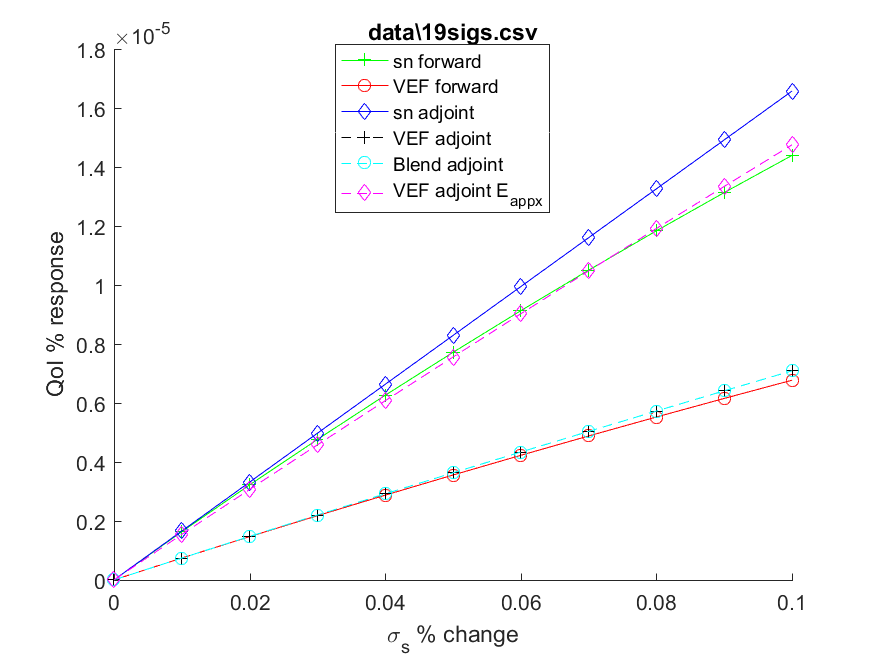
\includegraphics[width=.98\linewidth]{figures/19sigsSens.png}
  \caption{Unperturbed state: $\sigt=2$, $\sigs=1$.}
  \label{fig:sfig1}
\end{subfigure}%
\\
\begin{subfigure}{.5\textwidth}
  \centering
  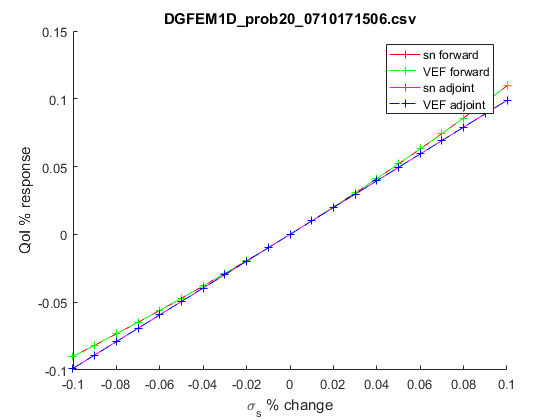
\includegraphics[width=.98\linewidth]{figures/20sigsSens.png}
  \caption{Unperturbed state: $\sigt=1$, $\sigs=0.5$.}
  \label{fig:sfig2}
\end{subfigure}
\\
\begin{subfigure}{.5\textwidth}
  \centering
  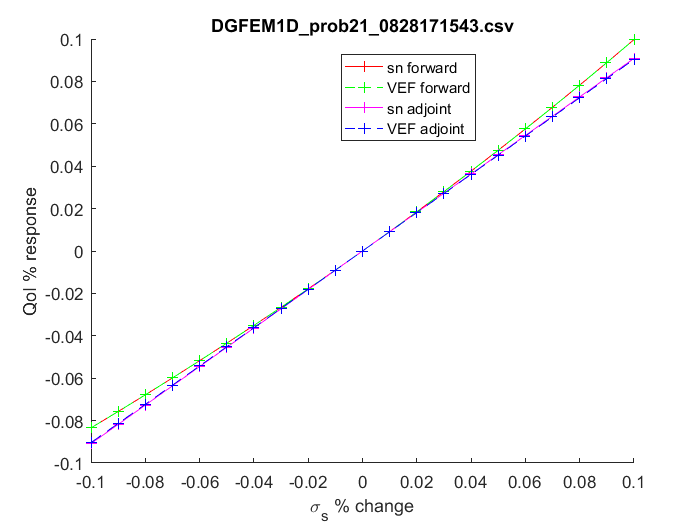
\includegraphics[width=.98\linewidth]{figures/21sigsSens.png}
  \caption{Unperturbed state: $\sigt=0.5$, $\sigs=0.25$.}
  \label{fig:sfig3}
\end{subfigure}
\caption{Plots of $\sigs$ perturbation sensitivity for uniformly perturbed system.}
\label{fig:fig}
\end{figure}

\begin{figure}[H]
\label{HomoPertq}
\centering
\begin{subfigure}{.65\textwidth}
  \centering
  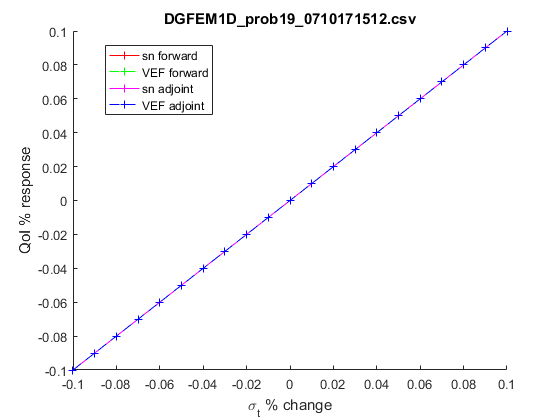
\includegraphics[width=.98\linewidth]{figures/19qSens.png}
  \caption{Unperturbed state: $\sigt=2$, $\sigs=1$}
  \label{fig:sfig1}
\end{subfigure}%
\\
\begin{subfigure}{.65\textwidth}
  \centering
  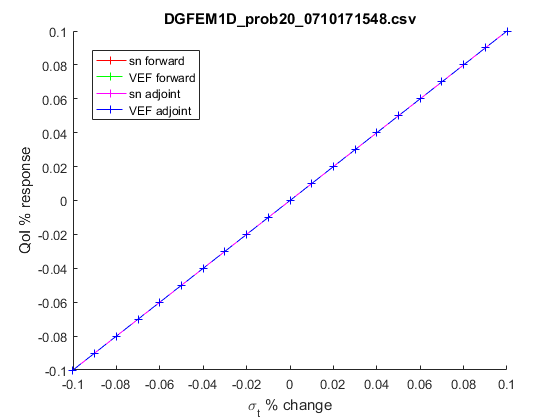
\includegraphics[width=.98\linewidth]{figures/20qSens.png}
  \caption{Unperturbed state: $\sigt=1$, $\sigs=0.5$}
  \label{fig:sfig2}
\end{subfigure}
\\
\begin{subfigure}{.65\textwidth}
  \centering
  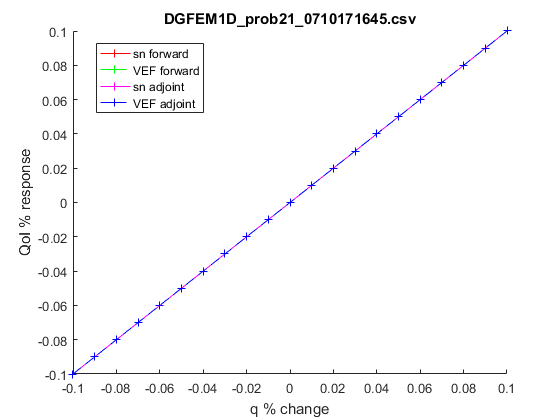
\includegraphics[width=.98\linewidth]{figures/21qSens.png}
  \caption{Unperturbed state: $\sigt=0.5$, $\sigs=0.25$}
  \label{fig:sfig3}
\end{subfigure}
\caption{Plots of source perturbation sensitivity for uniformly perturbed system.}
\label{fig:fig}
\end{figure}

\jcr{comment the results!}

\jcr{why no examples with changing the incident flux value?}

%%%%%%%----------------------------------------------------------------------------------------------
\subsection{Homogeneous initial system, Non-Uniform Perturbations}
%%%%%%%----------------------------------------------------------------------------------------------

The next test case has the same initial conditions as the previous homogeneous case. however the system is perturbed into a inhomogeneous system. The system is split into 5 equal widths. The first, third, and fifth sections (corresponding to the center and the end sections) have the relevant variable perturbed in one direction, while the other two segments are perturbed in the opposite direction. The result is a system that is inhomogeneous, but with regular variations and symmetric about the midpoint. The \qoi is also retained from the previous case.

\jcr{change the other figures/caption in the same manner as before}

\begin{figure}[H]
\label{InHomoPertt}
\centering
\begin{subfigure}{.65\textwidth}
  \centering
  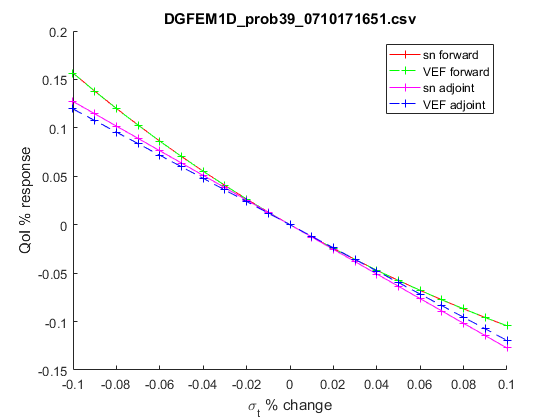
\includegraphics[width=.98\linewidth]{figures/39sigtSens.png}
  \caption{Unperturbed state: $\sigt=2$, $\sigs=1$}
  \label{fig:sfig1}
\end{subfigure}%
\\
\begin{subfigure}{.65\textwidth}
  \centering
  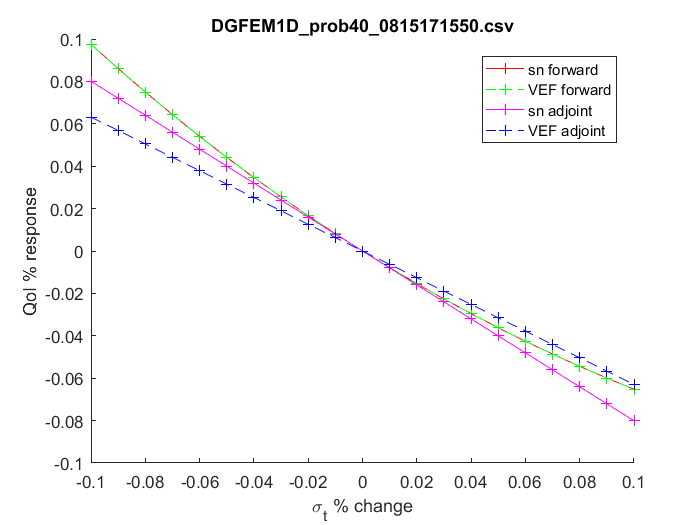
\includegraphics[width=.98\linewidth]{figures/40sigtSens.png}
  \caption{Unperturbed state: $\sigt=1$, $\sigs=0.5$}
  \label{fig:sfig2}
\end{subfigure}
\\
\begin{subfigure}{.65\textwidth}
  \centering
  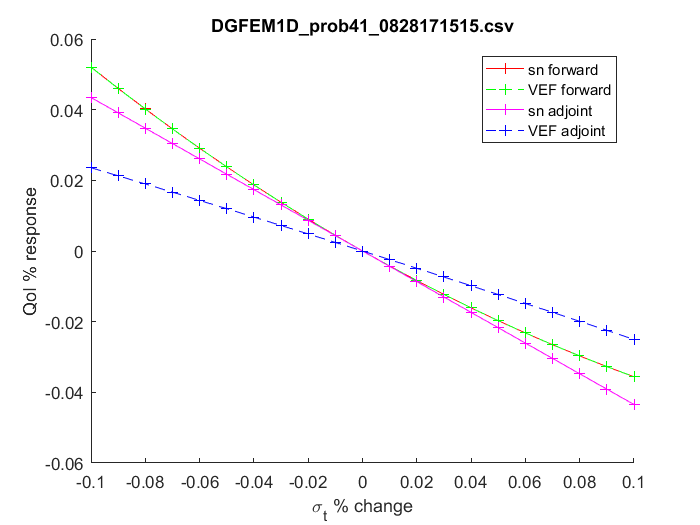
\includegraphics[width=.98\linewidth]{figures/41sigtSens.png}
  \caption{Unperturbed state: $\sigt=0.5$, $\sigs=0.25$}
  \label{fig:sfig3}
\end{subfigure}
\caption{Plots of $\sigt$ perturbation sensitivity for non-uniformly perturbed system.}
\label{fig:fig}
\end{figure}

\begin{figure}[H]
\label{InHomoPerts}
\centering
\begin{subfigure}{.65\textwidth}
  \centering
  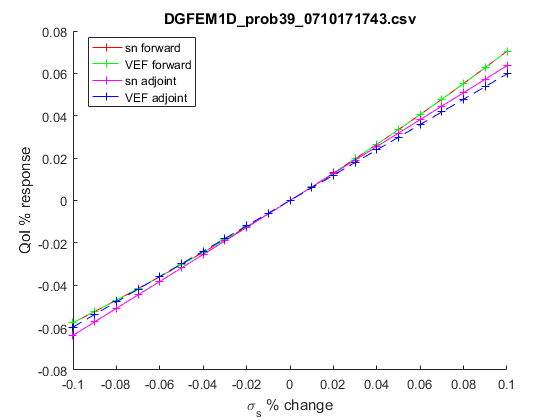
\includegraphics[width=.98\linewidth]{figures/39sigsSens.png}
  \caption{Unperturbed state: $\sigt=2$, $\sigs=1$}
  \label{fig:sfig1}
\end{subfigure}%
\\
\begin{subfigure}{.65\textwidth}
  \centering
  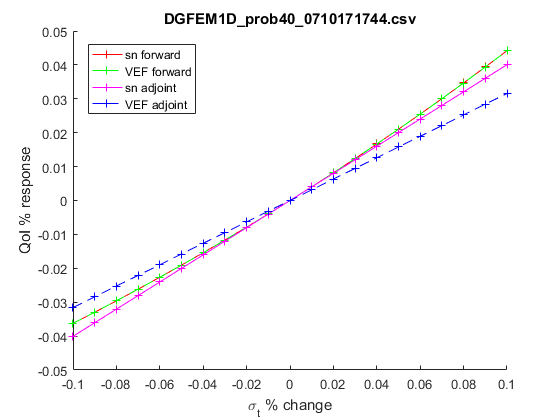
\includegraphics[width=.98\linewidth]{figures/40sigsSens.png}
  \caption{Unperturbed state: $\sigt=1$, $\sigs=0.5$}
  \label{fig:sfig2}
\end{subfigure}
\\
\begin{subfigure}{.65\textwidth}
  \centering
  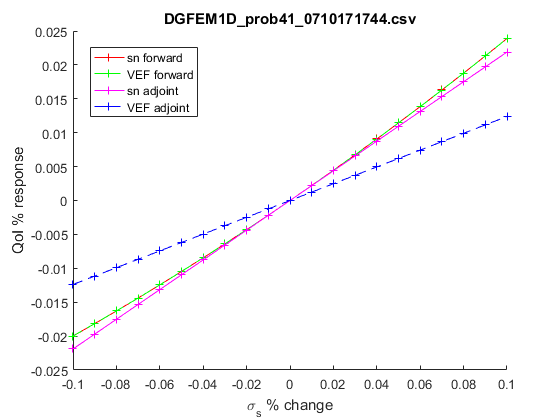
\includegraphics[width=.98\linewidth]{figures/41sigsSens.png}
  \caption{Unperturbed state: $\sigt=0.5$, $\sigs=0.25$}
  \label{fig:sfig3}
\end{subfigure}
\caption{Plots of $\sigs$ perturbation sensitivity for non-uniformly perturbed system.}
\label{fig:fig}
\end{figure}

\begin{figure}[H]
\label{InHomoPertq}
\centering
\begin{subfigure}{.65\textwidth}
  \centering
  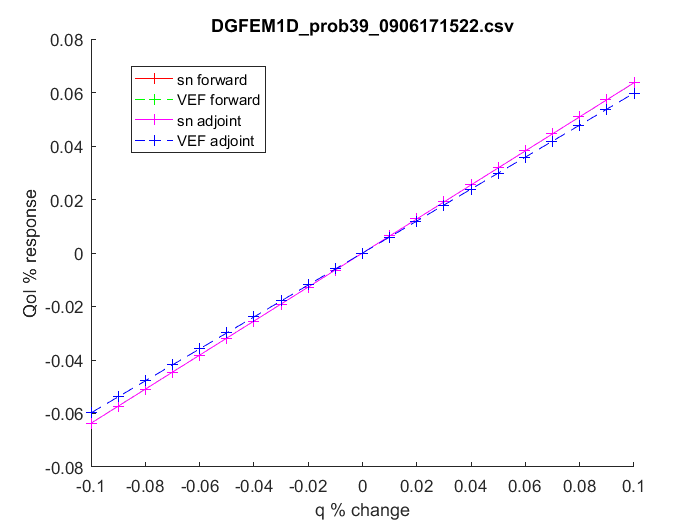
\includegraphics[width=.98\linewidth]{figures/39qSens.png}
  \caption{Unperturbed state: $\sigt=2$, $\sigs=1$}
  \label{fig:sfig1}
\end{subfigure}%
\\
\begin{subfigure}{.65\textwidth}
  \centering
  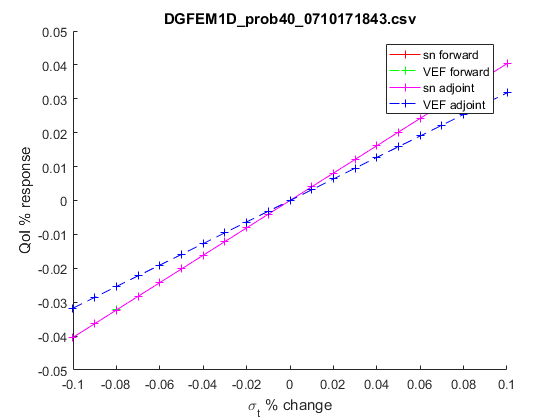
\includegraphics[width=.98\linewidth]{figures/40qSens.png}
  \caption{Unperturbed state: $\sigt=1$, $\sigs=0.5$}
  \label{fig:sfig2}
\end{subfigure}
\\
\begin{subfigure}{.65\textwidth}
  \centering
  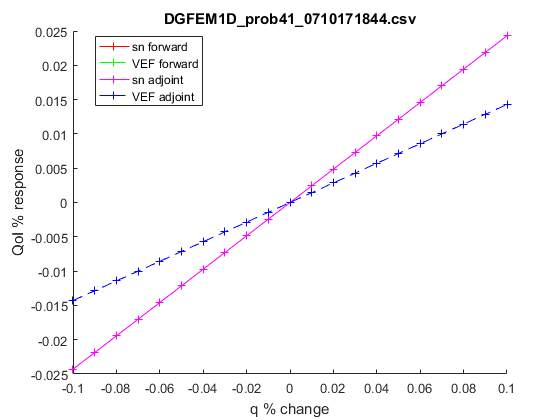
\includegraphics[width=.98\linewidth]{figures/41qSens.png}
  \caption{Unperturbed state: $\sigt=0.5$, $\sigs=0.25$}
  \label{fig:sfig3}
\end{subfigure}
\caption{Plots of source perturbation sensitivity for non-uniformly perturbed system.}
\label{fig:fig}
\end{figure}


\jcr{comment the results!}

\jcr{why no examples with changing the incident flux value?}



%%%%%%%----------------------------------------------------------------------------------------------
\subsection{Streaming system}
%%%%%%%----------------------------------------------------------------------------------------------
To generate a streaming system, we retain the 5 equal width sectioning of the previous inhomogeneous example, but the second and fourth sections are converted to streaming regions ($\sigt \approx 0 $). Leaving three neutron producing sections separated by two streaming gaps. The \qoi remains as the total neutron count in the center fifth section.

\jcr{same comments as above}

\begin{figure}[H]
\label{InHomoPertt}
\centering
\begin{subfigure}{.65\textwidth}
  \centering
  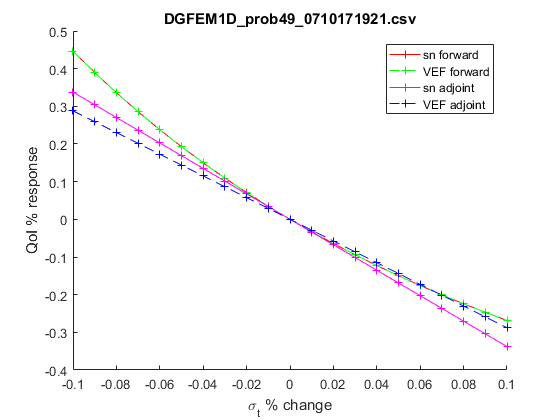
\includegraphics[width=.98\linewidth]{figures/49sigtSens.png}
  \caption{Unperturbed state: $\sigt=2$, $\sigs=1$}
  \label{fig:sfig1}
\end{subfigure}%
\\
\begin{subfigure}{.65\textwidth}
  \centering
  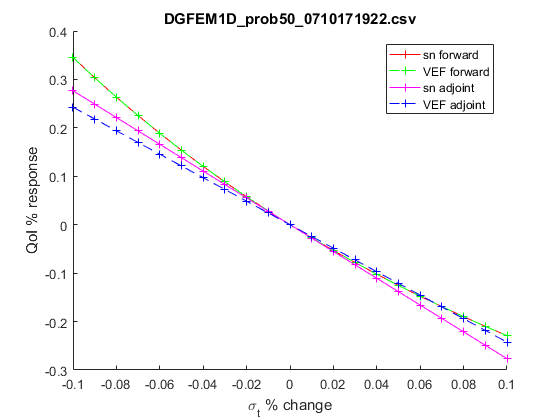
\includegraphics[width=.98\linewidth]{figures/50sigtSens.png}
  \caption{Unperturbed state: $\sigt=1$, $\sigs=0.5$}
  \label{fig:sfig2}
\end{subfigure}
\\
\begin{subfigure}{.65\textwidth}
  \centering
  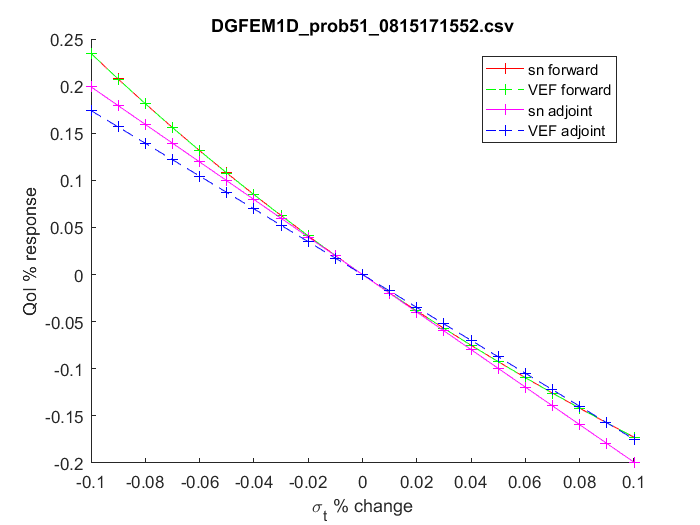
\includegraphics[width=.98\linewidth]{figures/51sigtSens.png}
  \caption{Unperturbed state: $\sigt=0.5$, $\sigs=0.25$}
  \label{fig:sfig3}
\end{subfigure}
\caption{Plots of $\sigt$ perturbation sensitivity for perturbed streaming system.}
\label{fig:fig}
\end{figure}

\begin{figure}[H]
\label{InHomoPerts}
\centering
\begin{subfigure}{.65\textwidth}
  \centering
  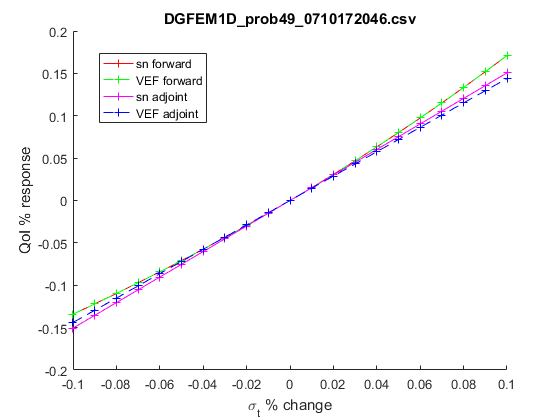
\includegraphics[width=.98\linewidth]{figures/49sigsSens.png}
  \caption{Unperturbed state: $\sigt=2$, $\sigs=1$}
  \label{fig:sfig1}
\end{subfigure}%
\\
\begin{subfigure}{.65\textwidth}
  \centering
  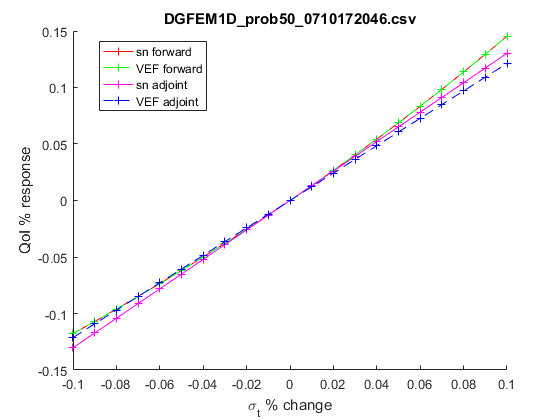
\includegraphics[width=.98\linewidth]{figures/50sigsSens.png}
  \caption{Unperturbed state: $\sigt=1$, $\sigs=0.5$}
  \label{fig:sfig2}
\end{subfigure}
\\
\begin{subfigure}{.65\textwidth}
  \centering
  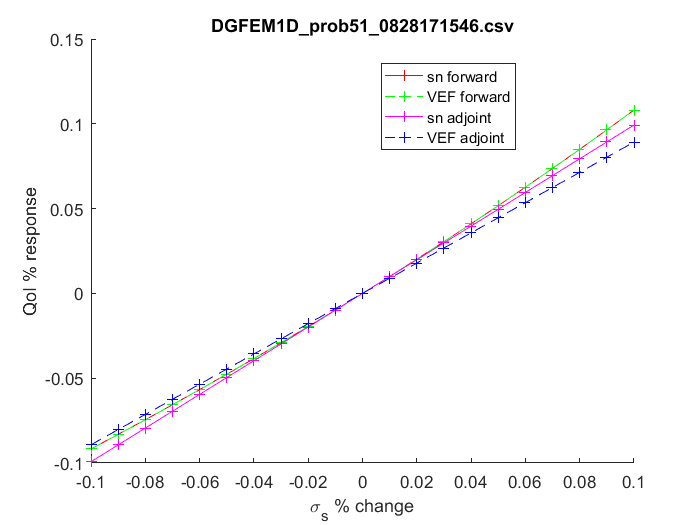
\includegraphics[width=.98\linewidth]{figures/51sigsSens.png}
  \caption{Unperturbed state: $\sigt=0.5$, $\sigs=0.25$}
  \label{fig:sfig3}
\end{subfigure}
\caption{Plots of $\sigs$ perturbation sensitivity for perturbed streaming system.}
\label{fig:fig}
\end{figure}

\begin{figure}[H]
\label{InHomoPertq}
\centering
\begin{subfigure}{.65\textwidth}
  \centering
  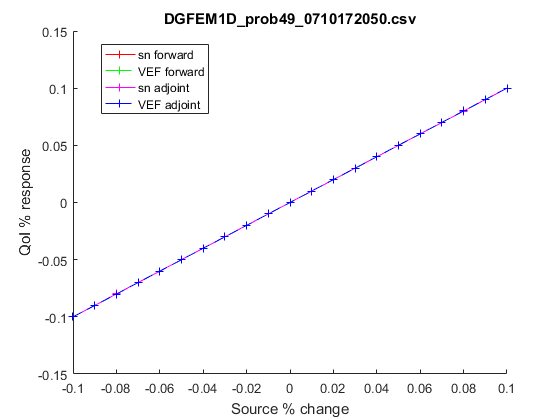
\includegraphics[width=.98\linewidth]{figures/49qSens.png}
  \caption{Unperturbed state: $\sigt=2$, $\sigs=1$}
  \label{fig:sfig1}
\end{subfigure}%
\\
\begin{subfigure}{.65\textwidth}
  \centering
  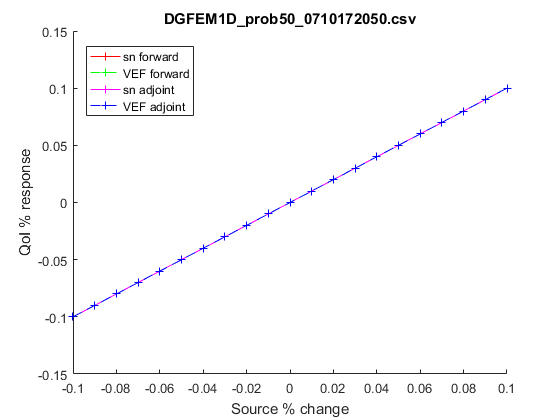
\includegraphics[width=.98\linewidth]{figures/50qSens.png}
  \caption{Unperturbed state: $\sigt=1$, $\sigs=0.5$}
  \label{fig:sfig2}
\end{subfigure}
\\
\begin{subfigure}{.65\textwidth}
  \centering
  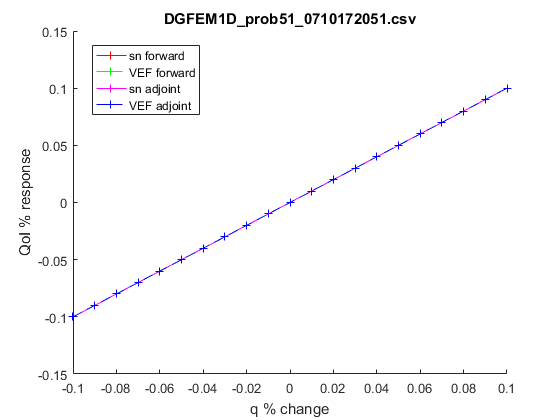
\includegraphics[width=.98\linewidth]{figures/51qSens.png}
  \caption{Unperturbed state: $\sigt=0.5$, $\sigs=0.25$}
  \label{fig:sfig3}
\end{subfigure}
\caption{Plots of source perturbation sensitivity for perturbed streaming system.}
\label{fig:fig}
\end{figure}
